\section{Part A}
\subsection{Technical Discussion}
Figure \ref{fig:original} shows a magnetic resonance image(MRI) of an upper thoracic human spine with a facture dislocation and spinal cord impingement. Because the original image is predominantly dark, an expansion of intensity levels is desirable. This can be accomplished with Log Transformation and Power-Low(Gamma) Transformation.
\begin{figure}[h]
\centering
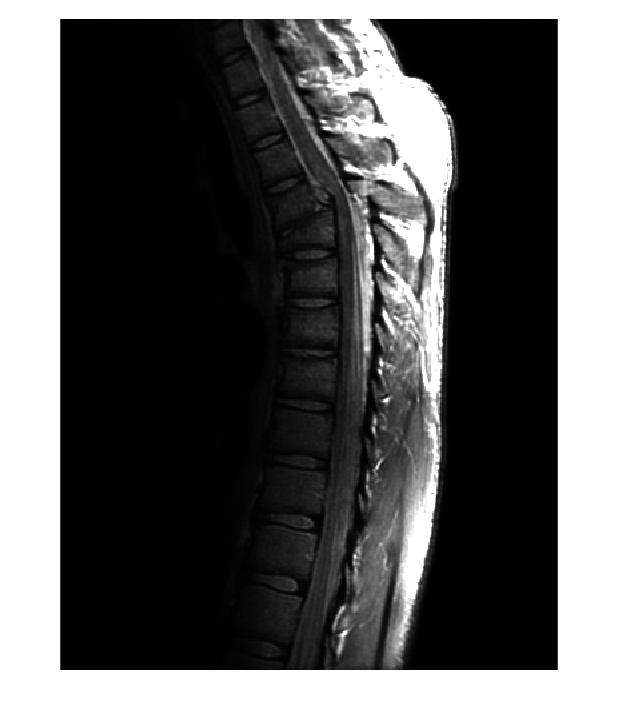
\includegraphics[scale=0.2]{0308}
\caption{Original Image}
\label{fig:original}
\end{figure}
\subsubsection{Log Transformations}
The general form of the log transformation is
$$ s=clog(1 + r) $$
where $r$ is the original pixel value between 0 and 1, $s$ is the pixel value after log transformation and $c$ is a constant. By observing the function we could find that this transformation maps a narrow range of low intensity values in the input into a wider range of output levels. We could use this kind of transformation to expand the values of dark pixels in the given MRI and compressing the higher-level values, which could show the details of the fractured part more obvious. 
\subsubsection{Power-Low(Gamma) Transformations}
Power-law transformations have the basic form
$$ s = cr^{\gamma} $$
Where where $r$ is the original pixel value between 0 and 1 and $s$ is the pixel value after transformation. $c$ and $ \gamma $ are positive constants. By observing the equation we could find that power-law transformation also map a narrow range of dark input values into a wider range of output values. By analyzing, we could notice that when $\gamma > 1$, the produced image tend to be darker than the original image. However, when $\gamma < 1$, the produced image will show more details on dark area of original image. In the following experiments, we need to find appropriate $c$ and $\gamma$ to show more details of the given MRI.
\subsection{Discussion of Results}
\subsubsection{Experiments of Log Transformations}
The experiments results of log transformation shows below:
\begin{figure}[h]
	\centering
	\subfloat[Subfigure 1 list of figures text][Original Image]{
		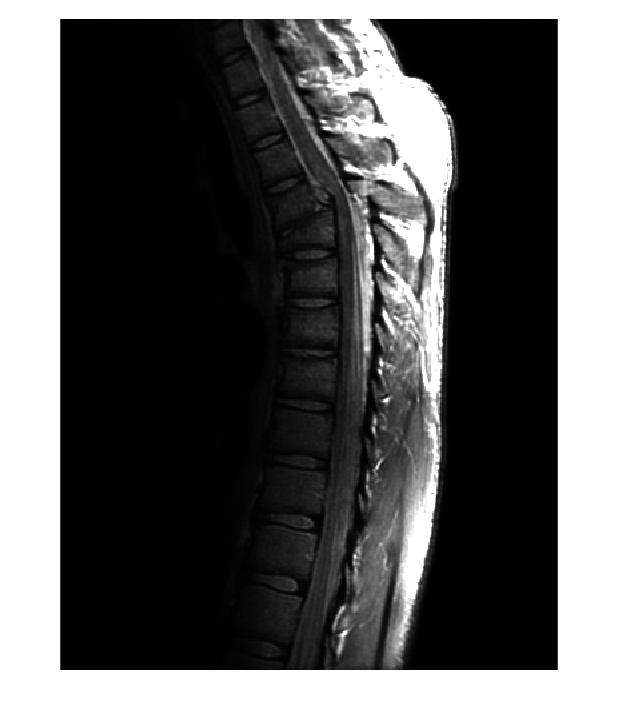
\includegraphics[width=0.2\textwidth]{0308}
		\label{fig:subfig1}}
	\subfloat[Subfigure 2 list of figures text][$c=1$]{
		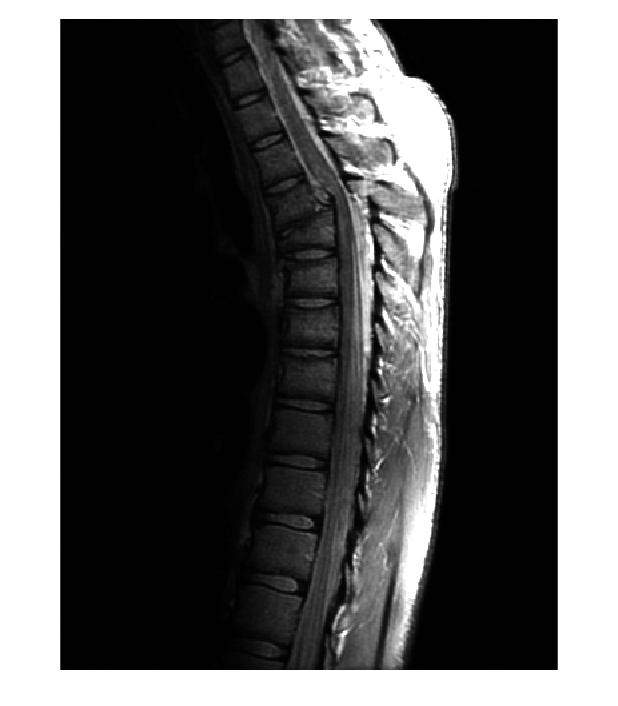
\includegraphics[width=0.2\textwidth]{logc1}
		\label{fig:subfig2}}
	\subfloat[Subfigure 3 list of figures text][$c=3$]{
		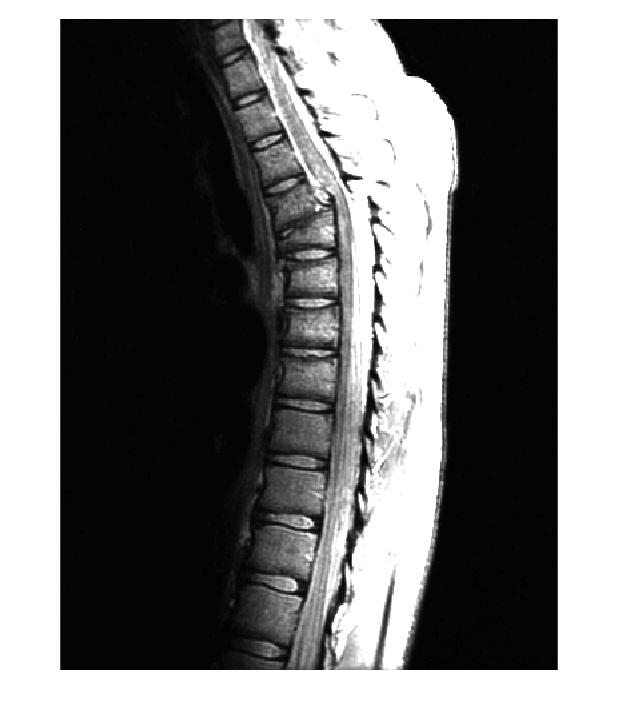
\includegraphics[width=0.2\textwidth]{logc3}
		\label{fig:subfig3}}
	\subfloat[Subfigure 4 list of figures text][$c=6$]{
		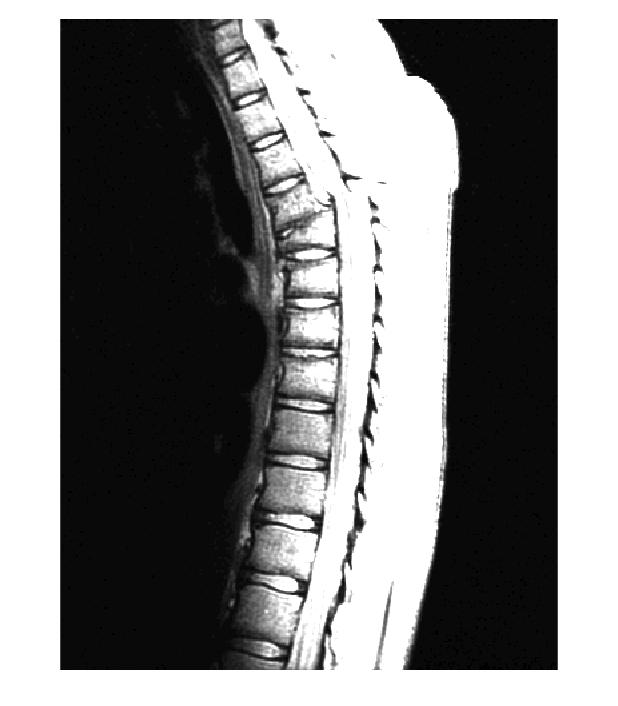
\includegraphics[width=0.2\textwidth]{logc6}
		\label{fig:subfig4}}
	\label{fig:exlogfig}
	\caption{Experiments results of log transformation when $c=$ 1, 3 and 6}
\end{figure}
As shown in Figure \ref{fig:subfig2}, the produced image shows more details on the dark area compare with the given MRI. However, the fractured area on the dark side still not clear enough. When we have $c=6$, we could find even more details on the dark area as it shows in Figure \ref{fig:subfig4}. But we could also notice that those area around the fractured point become totally white, which may result in missing of important information. As shown in Figure \ref{fig:subfig3} When $c=3$, we could have a relative desirable output image since it provides us enough information about the fracture also dark area. 
\begin{figure}[h]
\centering
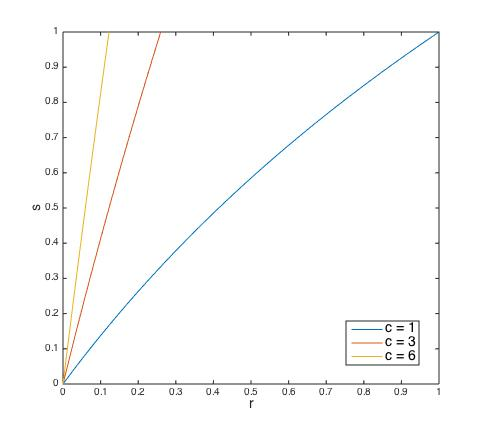
\includegraphics[scale=0.4]{log136}
\caption{The curve of $clog(r + 1)$ when $c =$ 1, 3 and 6}
\label{fig:curvelog}
\end{figure}
The reason behind it could be found in Figure \ref{fig:curvelog}. So, when $c=3$ the output image could have best visual enhancement.
\subsubsection{Experiments of Power-Low Transformations}





